\section{JugandoSudoku}

1. Al iniciar la aplicación la tabla de Sudoku aparece encerada, de la siguiente manera:

\begin{figure}[htbp]
\begin{center}
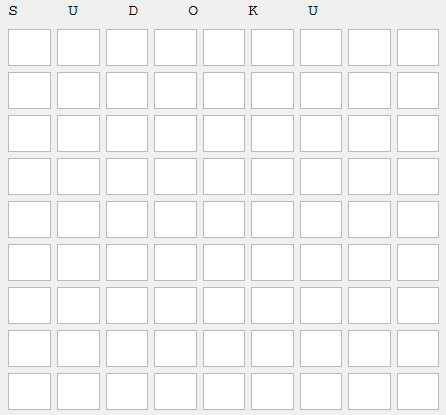
\includegraphics[width=.42\textwidth]{./imagenes/Tabla.png}
\caption{Tabla}
\label{Tabla}
\end{center}
\end{figure}


2. Para empezar una nueva partida, primero escogemos el nivel de dificultad (Figura 5.4), luego escogemos la opción NUEVO JUEGO (Figura 5.3). \\ Entonces nos aparecerá la tabla de Sudoku con celdas resueltas y celdas vacías (Dependiendo del Nivel de Dificultad aparacerán menos casillas vacías si el nivel escogido es Juvenil, y más casillas vacias si el nivel es más avanzado).


\begin{figure}[htbp]
\begin{center}
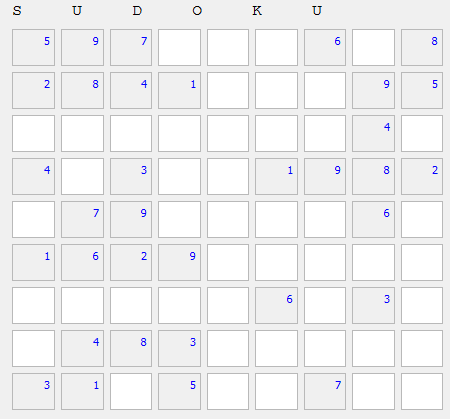
\includegraphics[width=.42\textwidth]{./imagenes/Tabla1.png}
\caption{Tabla1}
\label{Tabla1}
\end{center}
\end{figure}


3. Mientras se esta resolviendo alguna partida de SUDOKU se podrán realizar diversidad de acciones dependiendo de las opciones que vaya escogiendo el usuario: 

\begin{center}
- Si escogemos la opción BORRAR JUEGO (Figura 5.3), la tabla del Sudoku se encera (Figura 5.7). 
\ \\ \ \\ 

- Si escogemos la opcion NUEVO JUEGO (Figura 5.3)  se borrá el avance de la solución actual propuesta por el usuario y se inicia una nueva partida (Figura 5.8). 
\ \\ \ \\ 

- Si seleccionamos la opción de ALERTA DE JUGADA INVALIDA, cada vez que digitemos un valor incorrecto la aplicación mostrará una alerta, mientras que si seleccionamos la opcion ALERTA DE JUGADAS INCORRECTAS, la aplicación nos mostrará alertas en todas las casillas en que este un valor incorrecto de la siguiente manera:
\end{center} 
 
\begin{figure}[htbp]
\begin{center}

\includegraphics[width=.60\textwidth]{./imagenes/NoDisponible.png}
\caption{ImagenPendiente}
\label{ImagenPendiente}
\end{center}
\end{figure}

\begin{center}
- En cualquier instancia de la partida podemos guardar la partida o cargar una partida que ha sido anteriormente guardada. 
\ \\ \ \\ 

- Si queremos visualizar la solución del Juego, seleccionamos la opción RESOLVER JUEGO (Figura 5.3) y la aplicación muestra la solución del Juego y la partida termina.
\end{center} 

\begin{figure}[htbp]
\begin{center}
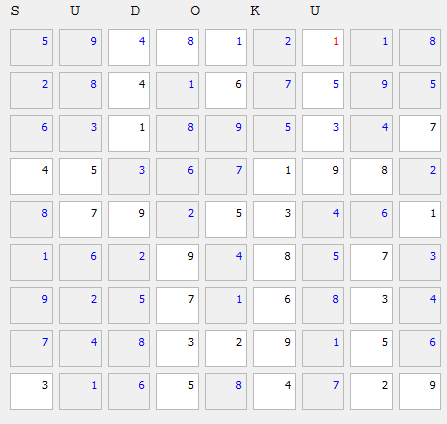
\includegraphics[width=.50\textwidth]{./imagenes/JuegoResuelto.png}
\caption{Juego Resuelto}
\label{Juego Resuelto}
\end{center}
\end{figure}

4. Si hemos terminado de resolver la partida por nuestra cuenta, procedemos a seleccionar lo opción COMPROBAR (Figura 5.3) y dependiendo de que si la solución es correcta o incorrecta la aplicación mostrará el siguiente mensaje:

\begin{figure}[htbp]
\begin{center}

\includegraphics[width=.50\textwidth]{./imagenes/NoDisponible.png}
\caption{ImagenPendiente}
\label{ImagenPendiente}
\end{center}
\end{figure}

\ \\ \ \\ \ \\ \ \\

5. Por último si deseamos observar las mejores partidas jugadas procedemos a seleccionar la opción SCORE DE PARTIDAS.

\begin{figure}[htbp]
\begin{center}

\includegraphics[width=.50\textwidth]{./imagenes/NoDisponible.png}
\caption{ImagenPendiente}
\label{ImagenPendiente}
\end{center}
\end{figure}


